\documentclass[crop,tikz,convert={outext=.svg,command=\unexpanded{pdf2svg \infile\space\outfile}},multi=false]{standalone}[2012/04/13]
\usepackage{tikz}
\usepackage{pgfplots}

\usetikzlibrary{arrows,shapes,positioning}
\begin{document}
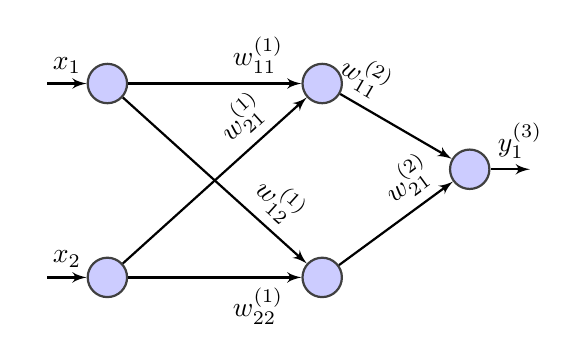
\begin{tikzpicture}[->,>=latex',shorten >=0pt,auto,node distance=2.2cm,
                    thick]
\tikzstyle{komp}=[rectangle,thick,draw=black!75,fill=black!0,minimum size=10mm]
\tikzstyle{sum_punkt}=[circle,thick,draw=black!75,fill=black!0,minimum size=3mm]
\tikzstyle{black_point}=[circle,thick,inner sep=0pt,draw=black!75,fill=black!100,minimum size=1mm]
\tikzstyle{get}=[circle,thick,draw=black!75,fill=black!0,minimum size=5mm]
\tikzstyle{agt}=[rectangle,thick,draw=black!75,fill=blue!25,minimum size=10mm]
\tikzstyle{komp2}=[rectangle,thick,draw=black,minimum size=10mm]
\tikzstyle{mot2}=[circle,thick,draw=black!75,fill=blue!20,minimum size=5mm]

\node[] (black_point_vor_regler) {};
\node[] (black_point_vor_regler1) [below=of black_point_vor_regler] {};

\node[mot2, align=center] (input1) [right=0.5cm of black_point_vor_regler]{};
\node[mot2, align=center] (input2)[right=0.5cm of black_point_vor_regler1] {};
\node[mot2, align=center] (hidden1)[right=of input1] {};
\node[mot2, align=center] (hidden2)[right=of input2] {};
\node[mot2, align=center] (output)[above right=1.0cm and 1.5cm of hidden2] {};
\node[] (ghostoutput) [right=0.5cm of output] {};

\draw[->](input1)-- node[near end,above] {$w^{(1)}_{11}$} (hidden1);
\draw[->](input1)--node[near end, sloped] {$w^{(1)}_{12}$}(hidden2);
\draw[->](input2)--node[near end, sloped] {$w^{(1)}_{21}$}(hidden1);
\draw[->](input2)--node[near end, below] {$w^{(1)}_{22}$}(hidden2);
\draw[->](hidden1)--node[pos=0.1, sloped] {$w^{(2)}_{11}$}(output);
\draw[->](hidden2)--node[near end, sloped] {$w^{(2)}_{21}$}(output);

\draw[->] (black_point_vor_regler) -- node[midway] {$x_1$} (input1);
\draw[->] (black_point_vor_regler1) -- node[midway] {$x_2$} (input2);
\draw[->] (output) -- node[near end] {$y^{(3)}_1$} (ghostoutput);
\end{tikzpicture}
\end{document}